%
% tangentialebene.tex
%
% (c) 2024 Prof Dr Andreas Müller
%
\begin{figure}
\centering
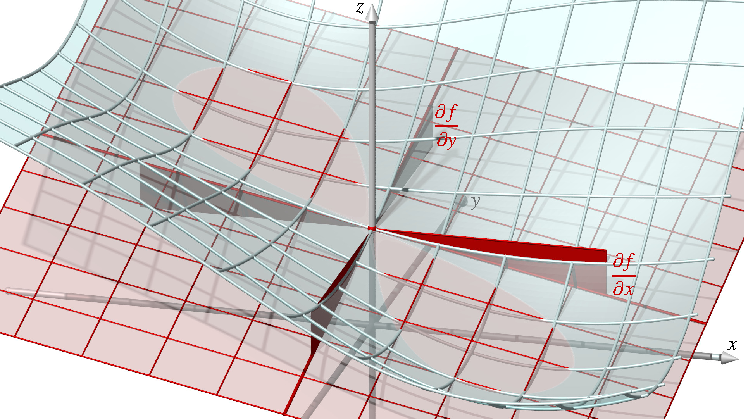
\includegraphics{chapters/010-fuvar/images/tangential.pdf}
%\includegraphics{chapters/010-fuvar/images/tangentialebene.pdf}
\caption{Mit den partiellen Ableitungen $\frac{\partial f}{\partial x}$
und $\frac{\partial f}{\partial y}$ einer Funktion lässt sich die rote
Tangentialebene in einem Punkt als lineare Ersatzfunktion konstruieren.
\label{buch:fuvar:richtungsableitung:fig:tangentialebene}}
\end{figure}
